%!TEX ROOT=ctutest.tex
\chapter{HW Design}
    Tato kapitola popisuje výběr použitého hardwaru a návrh měřicí a centrální jednotky.
\section{Měřicí jednotka (LoRa Node)}
\subsection{Výběr komponent}
\subsubsection{Mikrokontrolér (MCU)}
    Výběr výpočetní jednotky byl ovlivněn zejména dvěma požadavky – dostatečným výpočetním výkonem, který je třeba pro zpracování signálu z~akcelerometru a výpočet vibračních analýz, a nízkou spotřebou. Tyto požadavky jdou ovšem zcela proti sobě, a nakonec byly tak jako kompromis použity procesory z „low power“ série mikrokontrolérů od firmy STM – STM32L0xx.
    
    V první prototypu jednotky byl tento procesor použit ve verzi L073 s~64~piny – STM32L073RZ na vývojové desce Nucleo. Během dalšího vývoje byla zvolena verze L072 s 32 piny – STM32L072KZ, zejména díky nadbytečnému počtu pinů u L073RZ. Z hlediska vnitřní architektury, výkonnosti a samotného programování jsou ale čipy téměř totožné.
    
    \textbf{Specifikace MCU STM32L072KZ:}  \cite{manual:6}
    \begin{itemize}
            \item 32bitové RISC jádro ARM Cotex M0+
            \item 192 kB flash paměti, 20 kB RAM paměti
            \item HSI RC oscilátor 16 MHz, 32 kHz RTC oscilátor
            \item 12-bit ADC 1.14 Msps, 16 kanálů
            \item 4x USART, 1xLPUSART, 6x SPI, 3x $\text{I}^2\text{C}$
            \item 7 kanálů DMA kontroléru podporujících ADC, SPI, $\text{I}^2\text{C}$, USART, DAC\ldots
            \item proudový odběr ve STDBY módu \SI{0.29}{\micro\ampere}
        \end{itemize}
        
     \begin{figure} [!htp]
    	    \centering
    	    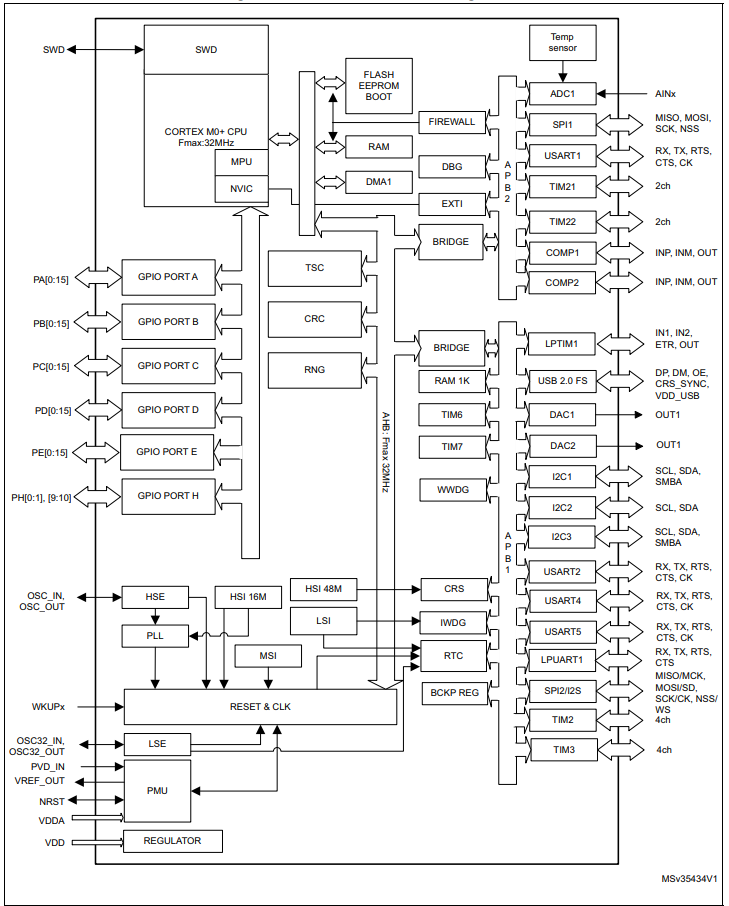
\includegraphics[ width =0.9\textwidth]{HW_PART/Figs/stm32l072xx.png}
            \caption {Blokový diagram MCU STM32L072xx. Převzato z \cite{manual:6}.}
    \end{figure} 
    


\subsubsection{LoRa modul}
\label{section:semtech_chips}
    Všechny čipy podporující modulaci sítě LoRa jsou vyvíjeny firmou Semtech, nesou označení SX a dělí se na dvě řady.\\
    První řada s čipy SX126x, SX127x, které se liší podle výkonnosti, nese označení \textit{LoRa Transceivers} a je určená pro koncové uzly. Tyto čipy neumožňují multikanálový příjem paketů a jsou omezeny na využití jednoho SF v danou chvíli. Naproti tomu druhá řada s čipy SX125x, SX13xx s označením \textit{LoRa Gateways} je mnohem výkonnější a umožňuje automatickou detekci SF přijatého signálu \cite{website:5}.
           
    Na trhu se nachází nepřeberné množství LoRa modulů, které se liší použitým LoRa čipem, tedy hlavně výstupním výkonem, podporou různých vlastností LoRa modulace a dále komunikačním rozhraním a cenou.\\
    Pro první prototyp měřicí jednotky byl nakonec použit LoRa modul přímo od firmy STM – \textbf{I-NUCLEO-SX1272D} s čipem SX1272, který byl součástí vývojářského kitu a který lze zapojit přímo do Nuclea \cite{software:2}.
          
    V druhé verzi byl využit velmi rozšířený modul  \textbf{RFM95W} s čipem SX1276, který se těší velké oblíbenosti především díky své nízké ceně.\\
    Problém nastal pouze u vysílacího výkonu, kdy modul RFM na rozdíl od referenční verze SX1276 neumožňuje použít RFO pin pro vysílání. Pro zesílení vysílaného paketu byl tak nakonec využit pin BOOST, který má ale výrazně vyšší spotřebu (více v \ref{table:currents}).
    
    
     \begin{figure} [!h]
        \centering
        \begin{subfigure}[b]{0.4\textwidth}
             \centering
             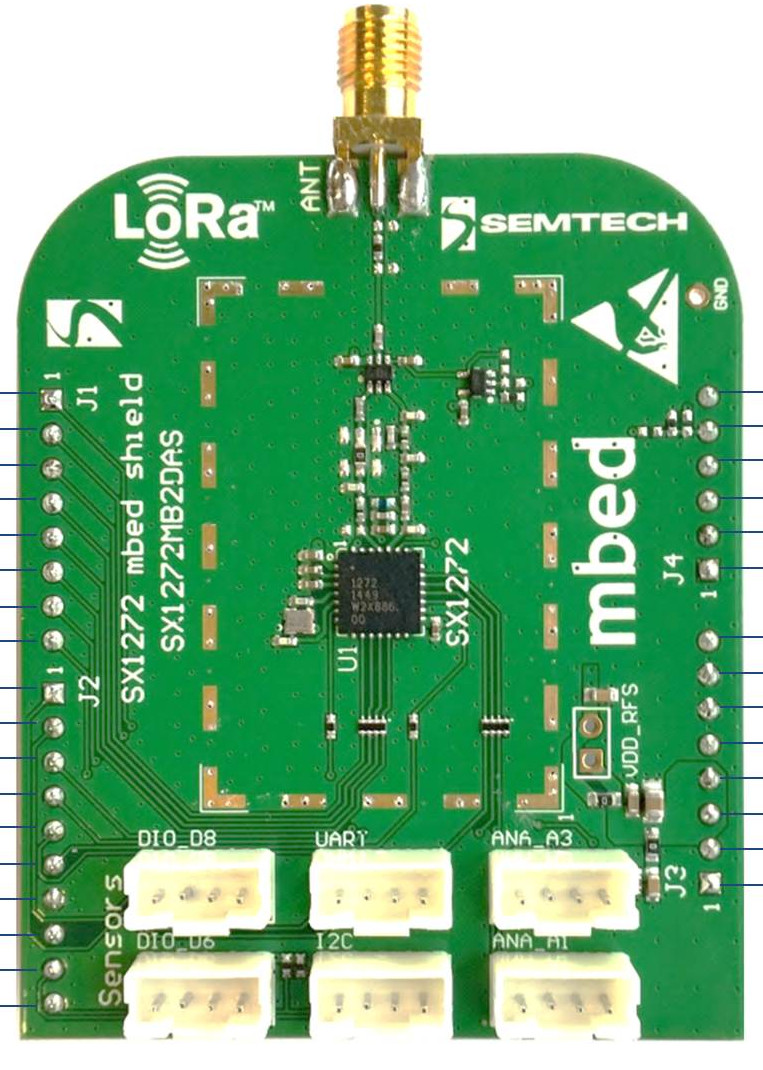
\includegraphics[width=\textwidth]{HW_PART/Figs/SX1272_pinout2.jpg}
             \caption {LoRa modul I-NUCLEO-SX1272D. Převzato z \cite{software:2}.}
         \end{subfigure}
         \hfill
        \begin{subfigure}[b]{0.4\textwidth}
            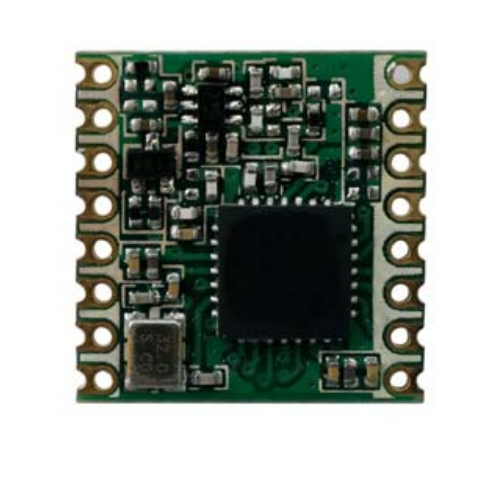
\includegraphics[ width =\textwidth]{HW_PART/Figs/rfm95W.png}
            \caption {LoRa modul RFM95W. Převzato z \cite{manual:5}.}
        \end{subfigure}
    \end{figure} 
    \textbf{Specifikace LoRa modulu RFM95W:} \cite{manual:5}
        \begin{itemize}
            \item link budget až 161 dB (rozdíl vysílacího výkonu a citlivosti přijímače) 
            \item programovatelný bitrate až 300 kbps
            \item vysílací výkon až +20 dBm (pro PA\_BOOST)
            \item citlivost až -148 dBm
            \item až 256bitové pakety
            \item proudový odběr v tabulce \ref{table:currents}
        \end{itemize}
    
        \begin{table}[H]
        \begin{ctucolortab}
        \begin{tabular}{c!{\vrule width 2pt}c}
            \textbf{Režim čipu} &  \textbf{Proudový odběr}\\ 
            \Xhline{4\arrayrulewidth}
            SLEEP mód & \SI{0.2}{\micro\ampere} \\\hline
            STDBY mód (RC oscilátor)& \SI{1.5}{\micro\ampere} \\\hline
            RX mód (LNA boost ON) & \SI{11.5}{\milli\ampere} \\\hline
            RX mód (LNA boost OFF) & \SI{10.8}{\milli\ampere} \\\hline
            TX mód (PA\_BOOST 20 dbm) & \SI{120}{\milli\ampere} \\\hline
            TX mód (PA\_BOOST 17 dbm) & \SI{87}{\milli\ampere} \\\hline
            TX mód (PA\_RFO 13 dbm) & \SI{29}{\milli\ampere} \\\hline
            TX mód (PA\_RFO 7 dbm) & \SI{20}{\milli\ampere}
        \end{tabular}
        \end{ctucolortab}
        \caption{Proudový odběr pro jednotlivé režimy čipu a vybrané vysílací výkony.}
        \label{table:currents}
    \end{table}

    

\subsubsection{Senzor vibrací}
    Výběr akcelerometru byl ovlivněný vhodností pro detekci vibračních signálů a nízkou spotřebou. Pro měření vibrací a to pouze v jedné ose kolmé na osu motoru (více o měření vibračního signálu v kapitole \ref{section:measuring}) postačoval jednoosý akcelerometr s šířkou pásma kolem deseti kilohertz, čemuž vyhovoval \textbf{ADXL1002} od firmy Analog Devices.\\
    Akcelerometr byl navíc dodán na vývojářské destičce  \textbf{EVAL-ADXL1002Z}, která je poměrně tlustá, odolná i vůči silným vibracím, dobře upevnitelná k~samotnému motoru a je na ní umístěn také RC filtr, který tlumí vyšší harmonické frekvence vznikající při modulaci signálu v senzoru a který zamezuje aliasingu.
    Analogový výstup akcelerometru je poté veden koaxiálním kabelem, jehož stínění potlačuje vliv vnějších rušivých polí na přenášený užitečný signál, a je následně zpracováván AD převodníkem na mikrokontroléru.
    
    \begin{figure} [!htp]
        \centering
        \begin{subfigure}[b]{0.48\textwidth}
             \centering
             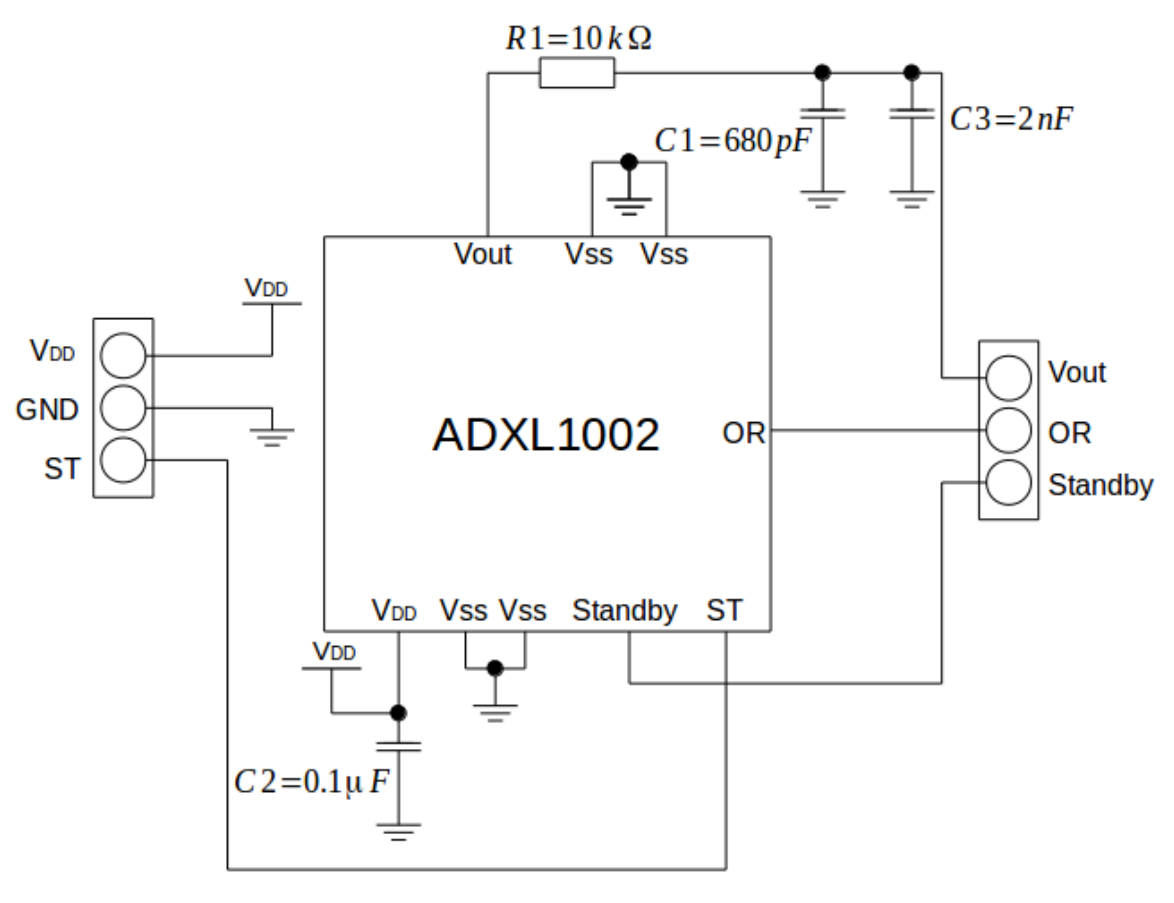
\includegraphics[width=\textwidth]{HW_PART/Figs/adxl1002.png}
             \caption {Schéma vývojové desky EVAL-ADXL1002Z. Převzato z \cite{manual:3}.}
         \end{subfigure}
         \hfill
        \begin{subfigure}[b]{0.49\textwidth}
            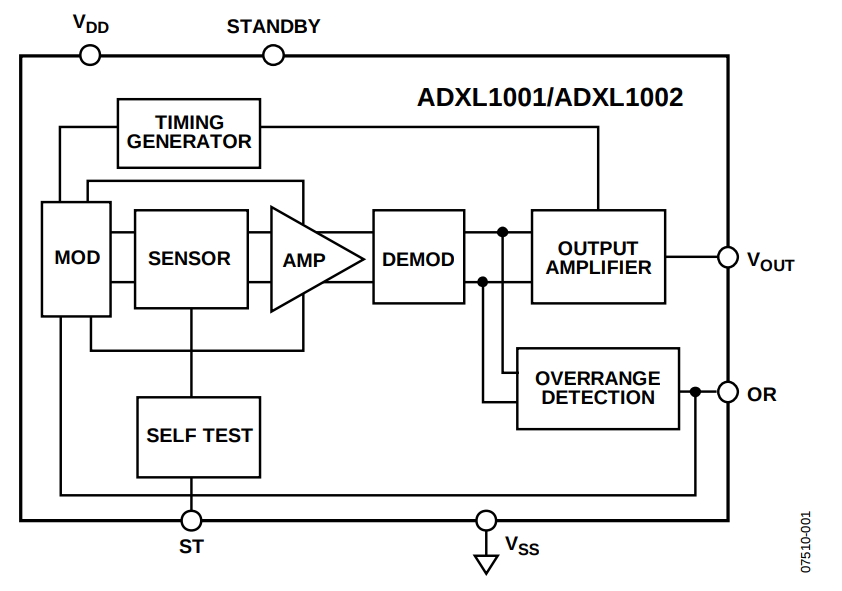
\includegraphics[ width =\textwidth]{HW_PART/Figs/adxl1002_functionaldiagram.png}
            \caption {Zjednodušený blokový diagram. Převzato z \cite{manual:3}.}
        \end{subfigure}
        \caption{Akcelerometr ADXL1002.}
    \end{figure} 
    
    \pagebreak
    
    \textbf{Specifikace akcelerometru ADXL1002:} \cite{manual:3}
        \begin{itemize}
            \item jednoosý akcelerometr typu MEMS (mikroelektromechanický)
            \item šířka pásma \SI{11}{\kilo Hz}
            \item měřicí rozsah \SI{\pm 50}{\textit{g}}
            \item citlivost \SI{40}{\milli V\textit{g}^{-1}}, při nulovém $g$ je na výstupu polovina napájecího napětí
            \item spektrální výkonová hustota šumu \SI{25}{\micro \textit{g}(\sqrt{Hz})^{-1}}
            \item analogový výstup
            \item proudový odběr v měřícím módu \SI{1}{\milli\ampere}
            \item proudový odběr v STDBY módu  \SI{225}{\micro\ampere}
        \end{itemize}
        
      \begin{figure} [!h]
        \centering
        \begin{subfigure}[!h]{0.6\textwidth}
             \centering
             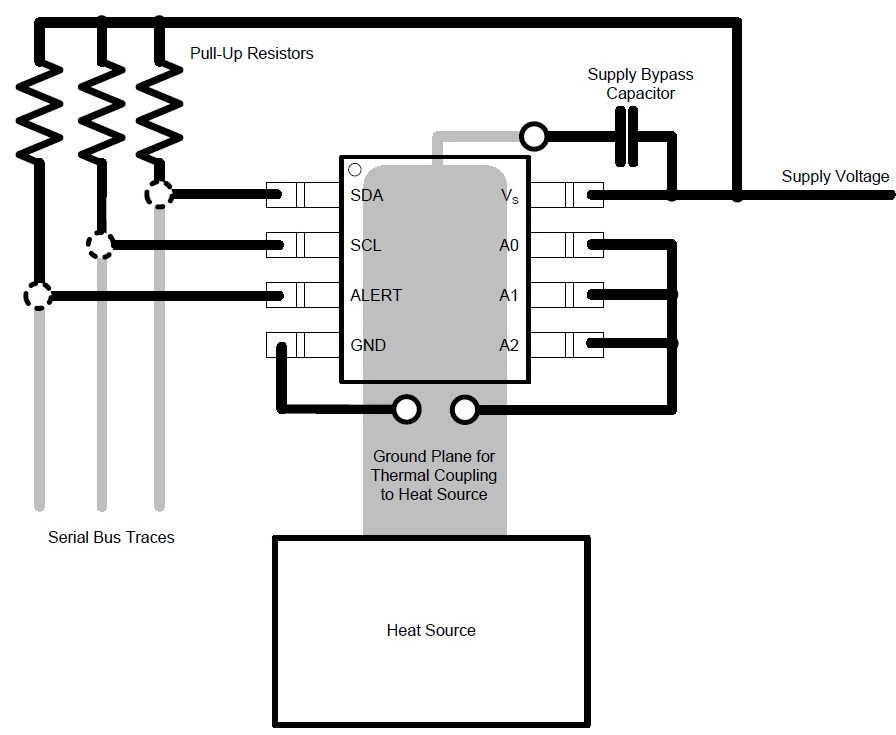
\includegraphics[width=\textwidth]{HW_PART/Figs/tmp75_connection.jpg}
             \caption {Schéma připojení TMP75. Převzato z \cite{manual:4}.}
         \end{subfigure}
         \hfill
        \begin{subfigure}[!h]{0.4\textwidth}
            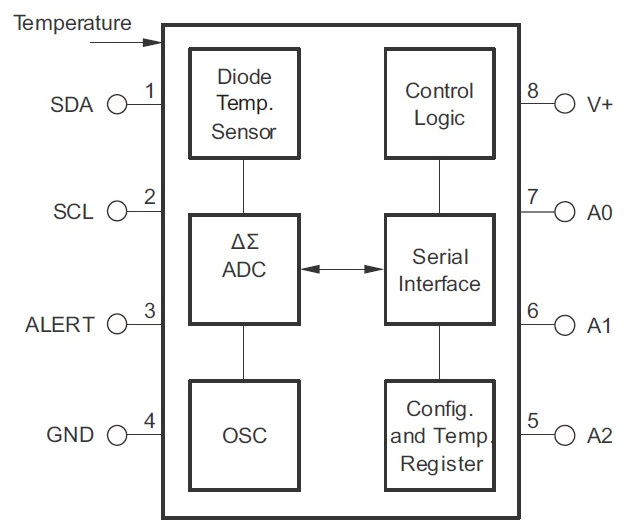
\includegraphics[ width =\textwidth]{HW_PART/Figs/tmp75.jpg}
            \caption {Zjednodušený blokový diagram TMP75. Převzato z \cite{manual:4}.}
        \end{subfigure}
        \caption{Teplotní senzor TMP75.}
    \end{figure} 
        

\subsubsection{Teplotní senzor}
    Pro monitorování teploty bylo vybráno digitální teplotní čidlo \textbf{TMP75} od firmy Texas Instruments, které pro měření využívá 12bitový převodník. Jedná se o poměrně rozšířený senzor komunikující po $\text{I}^2\text{C}$ sběrnici, který je díky své malé spotřebě vhodný zejména do zařízení, která jsou poháněna baterií.
    
    \textbf{Specifikace teplotního čidla TMP75:} \cite{manual:4}
        \begin{itemize}
            \item typ čidla výrobce neuvádí, zřejmě se jedná o měření teploty na PN přechodu tranzistoru
            \item přesnost \SI{\pm 1}{\degree C}
            \item programovatelné rozlišení 9-12 bitů
            \item rozsah \SI{-40}{\degree C}-\SI{+125}{\degree C}
            \item proudový odběr \SI{50} {\micro\ampere}
        \end{itemize}
        
       

     
 

\subsection{Celkový design} 

\subsubsection{První prototyp}
    První verze měřicí jednotky byla vytvořena pomocí vývojářského kitu Nucleo s~procesorem STM32L073RZ a LoRa modulem s čipem SX1272. Teplotní čidlo a akcelerometr byly do Nuclea připojeny pomocí 125 centimetrů dlouhých drátů, dostatečně dlouhých nato, aby se daly připevnit přímo na motor. Výstup akcelerometru byl veden koaxiálním kabelem. V obou dvou verzích  byla využita stejná anténa na 868 MHz se SMA konektorem, která byla dodána ve vývojářském kitu.
    První verzi měřicí jednotky lze vidět na obrázku \ref{figure:first_prototype}.

     \begin{figure} [!htp]
    	    \centering
    	    \includegraphics[ width =0.8\textwidth]{HW_PART/Figs/REAL/M_01.png}
            \caption {První verze měřicí jednotky.}
            \label{figure:first_prototype}
    \end{figure} 
    
\subsection{Druhá verze}
    Druhá verze měřicí jednotky byla vytvořena bez Nuclea zapájením čipu STM3272KZ na adaptor, stejně jako LoRa modulu RFM95W. Adaptory byly společně se stabilizačním obvodem, restartovacím tlačítkem, blokovacími kondenzátory a konektory pro připojení senzorů a programátoru připájeny k~univerzální pájecí destičce, jak lze vidět na obrázku \ref{figure:second_prototype}. Li-Pol baterie použitá k napájení zařízení měla kapacitu 1900 mAh a výstupní napětí 3.7 V. Schéma zapojení je znázorněno na obrázku \ref{figure:scheme_01}.
    \begin{figure} [!htp]
        \centering
        \includegraphics[ width =0.8\textwidth]{HW_PART/Figs/REAL/M_02.png}
        \caption {Druhá verze měřicí jednotky.}
        \label{figure:second_prototype}
    \end{figure} 





\section{Řídicí jednotka (LoRa Gateway)}
\subsection{Výběr komponent}
\subsubsection{Mikrokontrolér (MCU)}

    Vlastní LoRa brána může být postavena spíše minimalisticky za použití určitého mikrokontroléru, tedy se slabým výkonem, ale nízkou cenou a spotřebou – například jako další STM32 jednotka s Ethernet nebo WiFi modulem nebo pomocí oblíbeného vývojářského čipu ESP8266/ESP32. Opačným přístupem by bylo postavení brány s výpočetně silnějším počítačem a operačním systémem, tedy s velkým výkonem, ale vyšší cenou a spotřebou.\\
    Pro realizaci brány bylo ale nakonec použité \textbf{Raspberry Pi} verze 3 model B. 
    Motivací výběru Raspberry, po zvážení kritérií popsaných výše, byl zejména dostatečný výpočetní výkon, vývojářská podpora a výhody operačního systému. Spotřeba brány není tak důležité kritérium jako u koncových zařízení, protože brána může mít stálý síťový zdroj napájení.
    
    \textbf{Specifikace Raspberry Pi 3 model B:} \cite{manual:7}
    \begin{itemize}
        \item 64 bitový čtyřjádrový procesor Broadcom BCM2835 1.2 GHz, 1 GB RAM
        \item 40 externích GPIO pinů
        \item BCM43438 WLAN a Bluetooth
        \item 4 USB porty, HDMI, 3.5 mm jack
        \item microSD port
    \end{itemize}
     \begin{figure} [H]
    	    \centering
    	    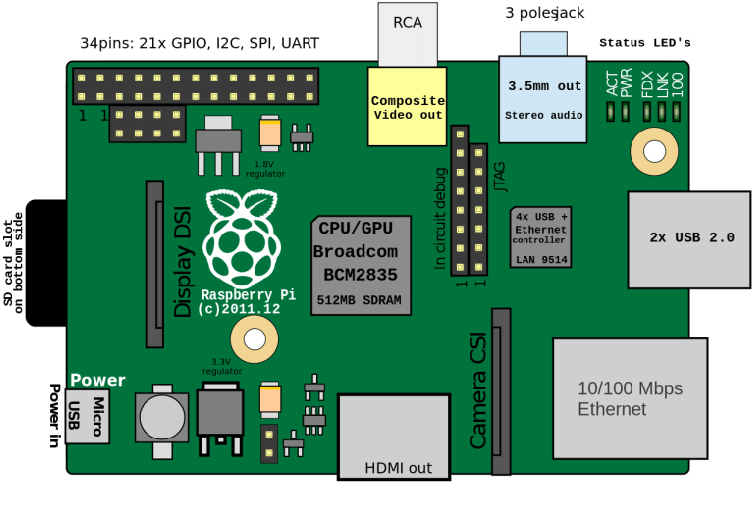
\includegraphics[ width = 0.65\textwidth]{HW_PART/Figs/rpi.png}
            \caption {Vybavení Raspberry Pi 3 model B. Převzato z \cite{manual:7}.}
    \end{figure} 
    
   
    
\subsubsection{LoRa modul}
    Z důvodů popsaných v kapitole \ref{section:single_channel_gw} byla brána navržena jako jednokanálová. Pro komunikaci tedy nebyly použity čipy ze série SX125x či SX13xx a v obou verzích byl využit stejný čip jako u měřicí jednotky – SX1272 v první verzi a RFM95W ve druhé verzi.
    \begin{figure} [!h]
    	    \centering
    	    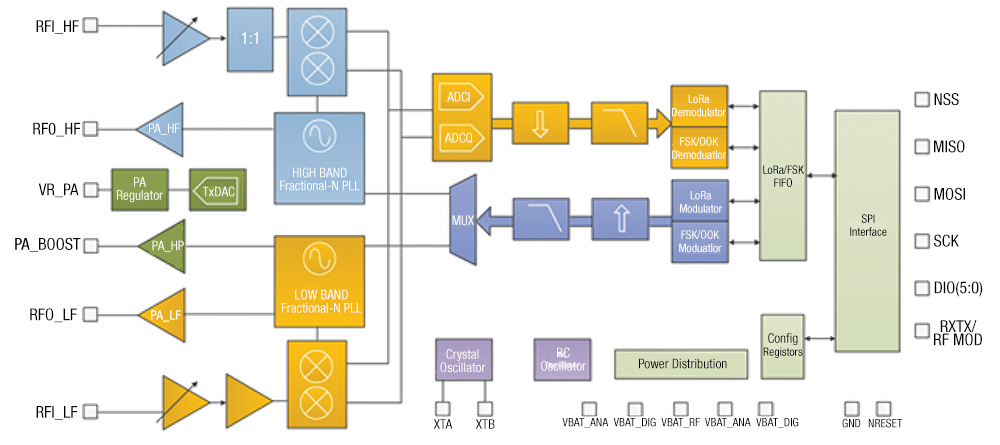
\includegraphics[ width =0.9\textwidth]{HW_PART/Figs/sx1276_block.jpg}
            \caption {Zjednodušený blokový diagram RFM95W.}
    \end{figure} 

\subsubsection{Displej}
    K Raspberry Pi byl připojen 7palcový dotykový displej s rozlišením 800 x 480. Skrz GPIO port bylo připojeno napájení 5 V a páskovým kabelem DSI port. 
    
    \begin{figure} [!hbp]
    	    \centering
    	    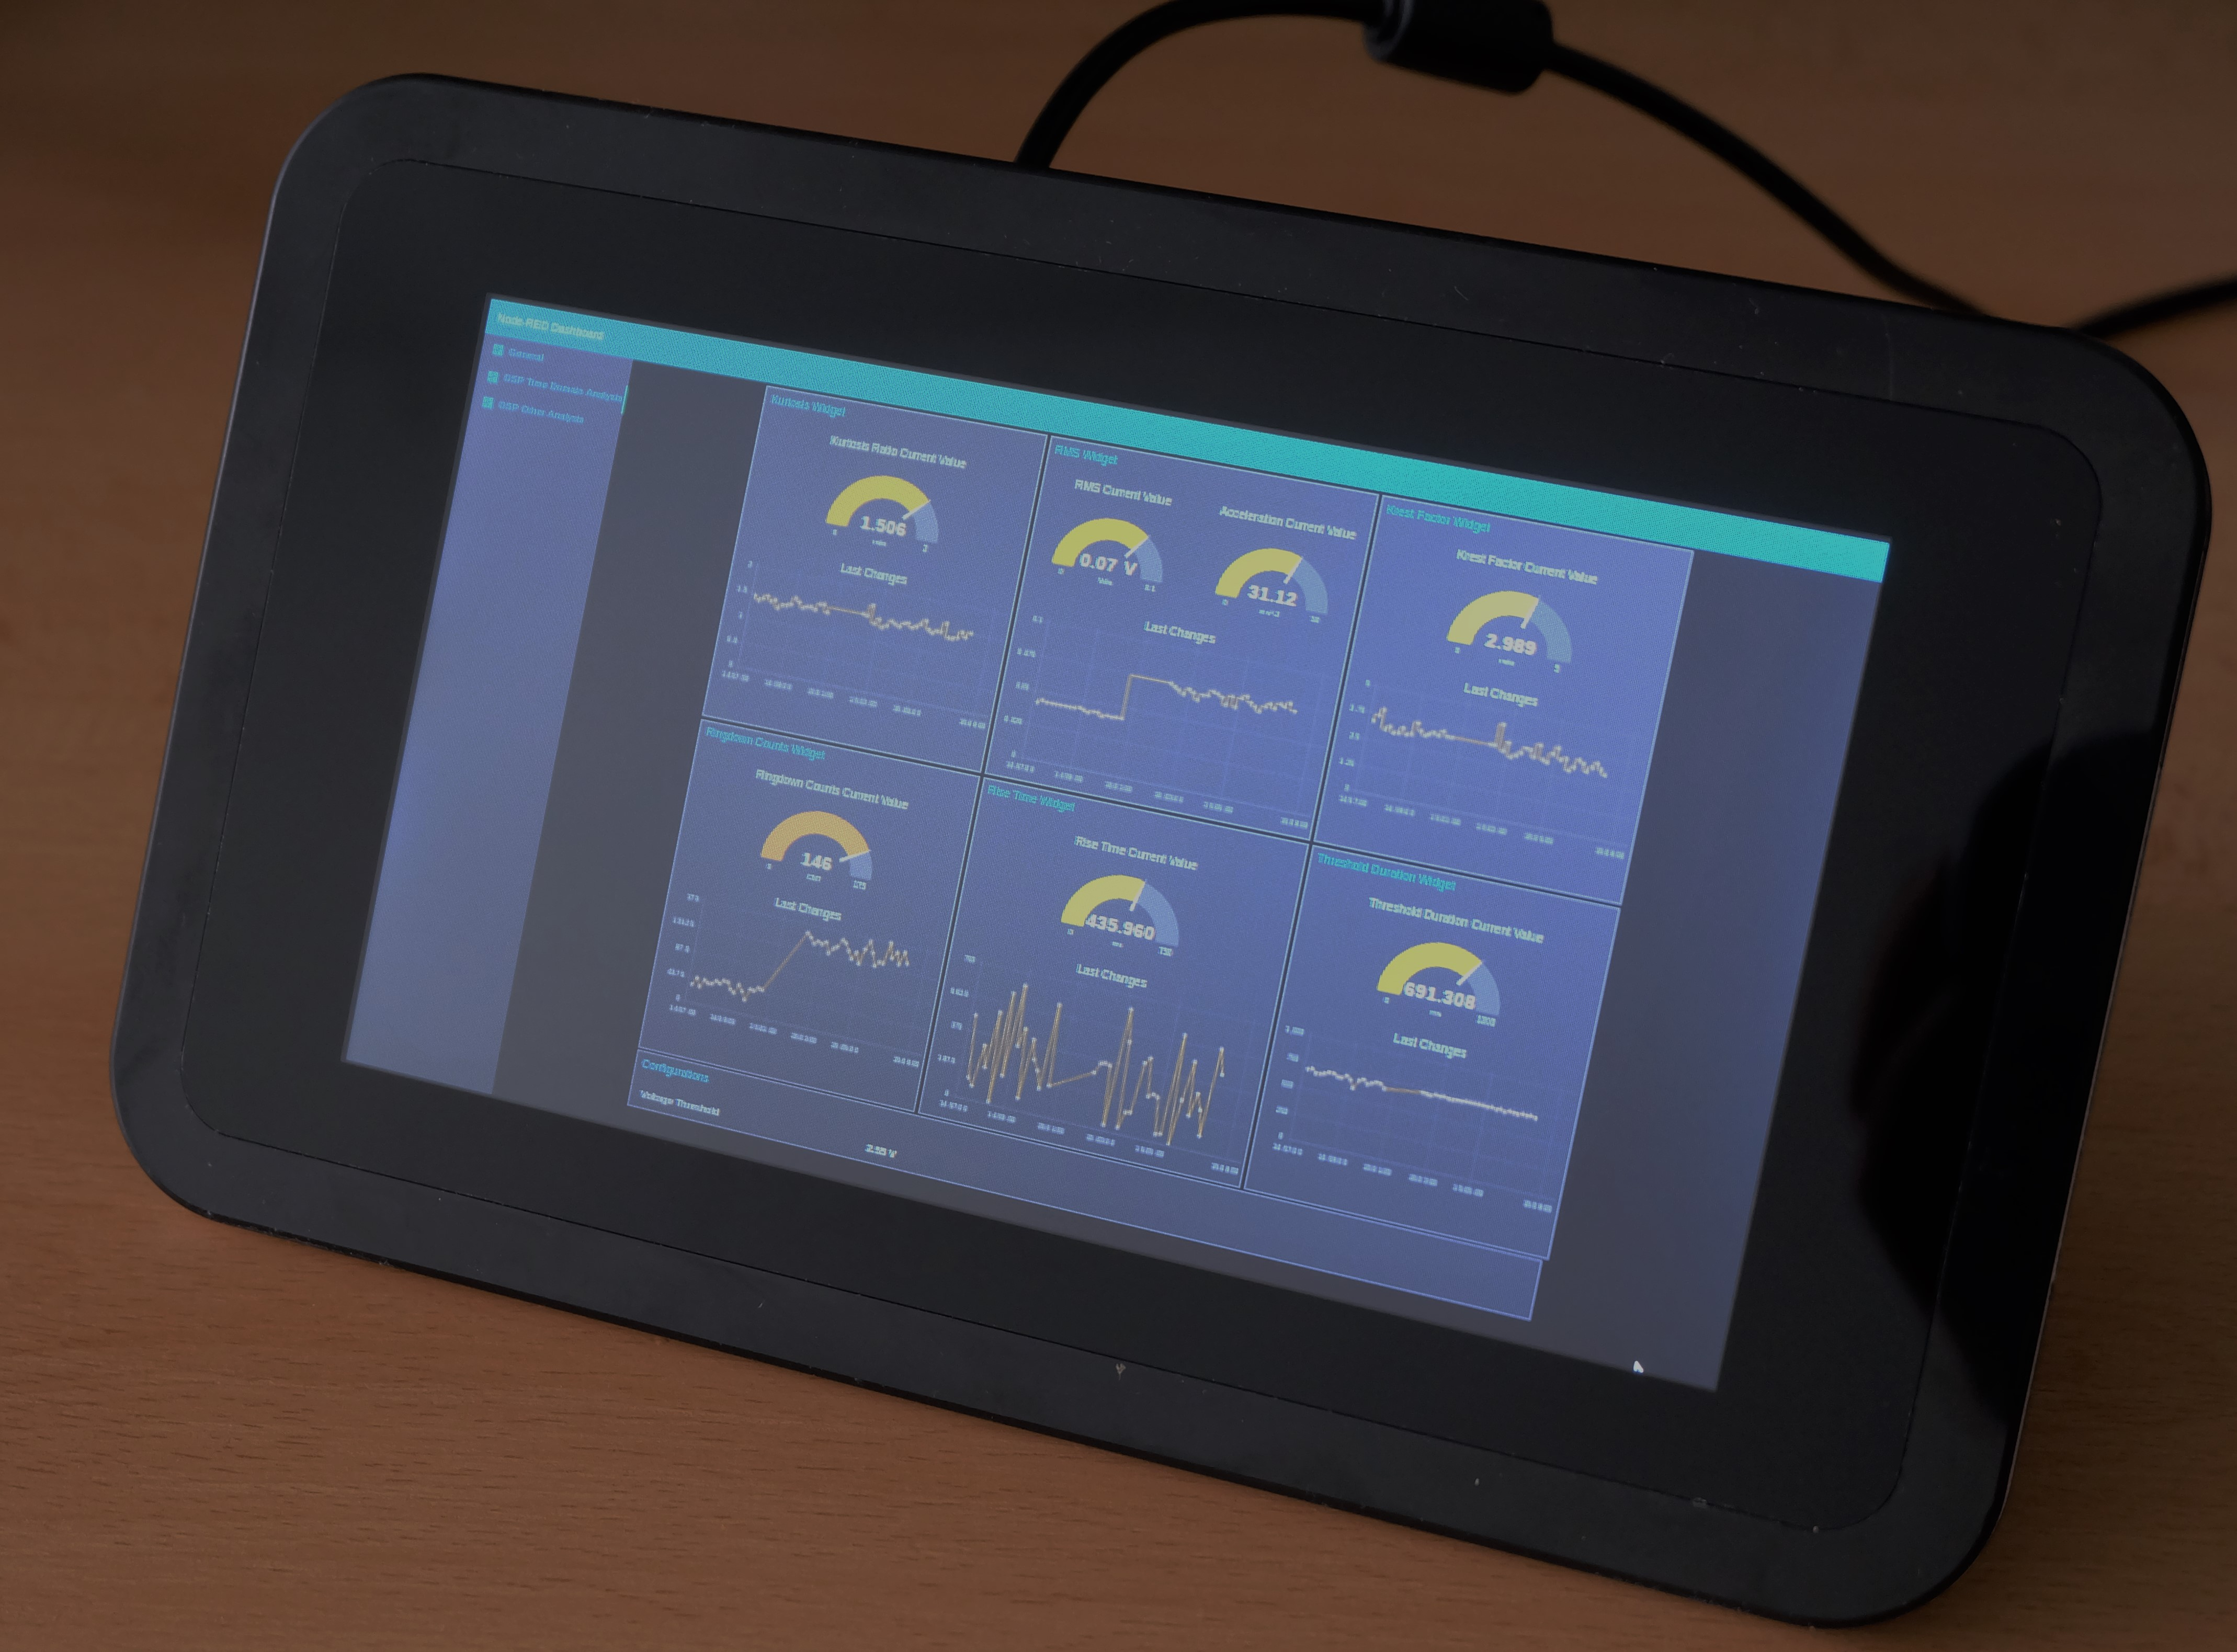
\includegraphics[ width =0.9\textwidth]{HW_PART/Figs/REAL/lcd.JPG}
            \caption {Centrální jednotka s připojeným dotykovým displejem.}
    \end{figure}
    
    Na displeji je po spuštění Raspberry automaticky zobrazeno uživatelské rozhraní popsané v kapitole \ref{section:gui} s časovými průběhy monitorovaných veličin.\\
    Motivací pro připojení displeje byl hlavně fakt, že v průmyslovém prostředí se může často hodit vidět průběhy analyzovaných veličin „naživo“ a rychle bez nutnosti připojovat se přes webovou stránku.
   

    
 \subsubsection{První prototyp}
    První verze brány byla vytvořena pouze s LoRa modulem určeným původně pro Nucleo I-NUCLEO-SX1272D, který musel být s GPIO piny Raspberry propojen jednotlivými drátky.
    \begin{figure} [!htp]
        \centering
        \includegraphics[ width =0.8\textwidth]{HW_PART/Figs/REAL/GW_01.png}
        \caption {První verze centrální jednotky.}
        \label{figure:first_prototype_gw}
    \end{figure} 
    
 \subsubsection{Druhá verze}
    Ve výsledné verzi byl použitý RFM95W LoRa modul. Pro jeho snadné připojení přímo do headru Raspberry byl vypůjčen návrh PCB, jehož autorem je student Ondřej Fidra \cite{book:3}.
    Výslednou verzi lze vidět na obrázku \ref{section:single_channel_gw}, schéma zapojení RFM95W do Raspberry na obrázku \ref{figure:scheme_02}.
    \begin{figure} [!ht]
        \centering
        \includegraphics[ width =0.8\textwidth]{HW_PART/Figs/REAL/GW_02.png}
        \caption {Druhá verze centrální jednotky.}
        \label{figure:second_prototype_gw}
    \end{figure} 
    
    \begin{figure} [!h]
    	    \centering
    	    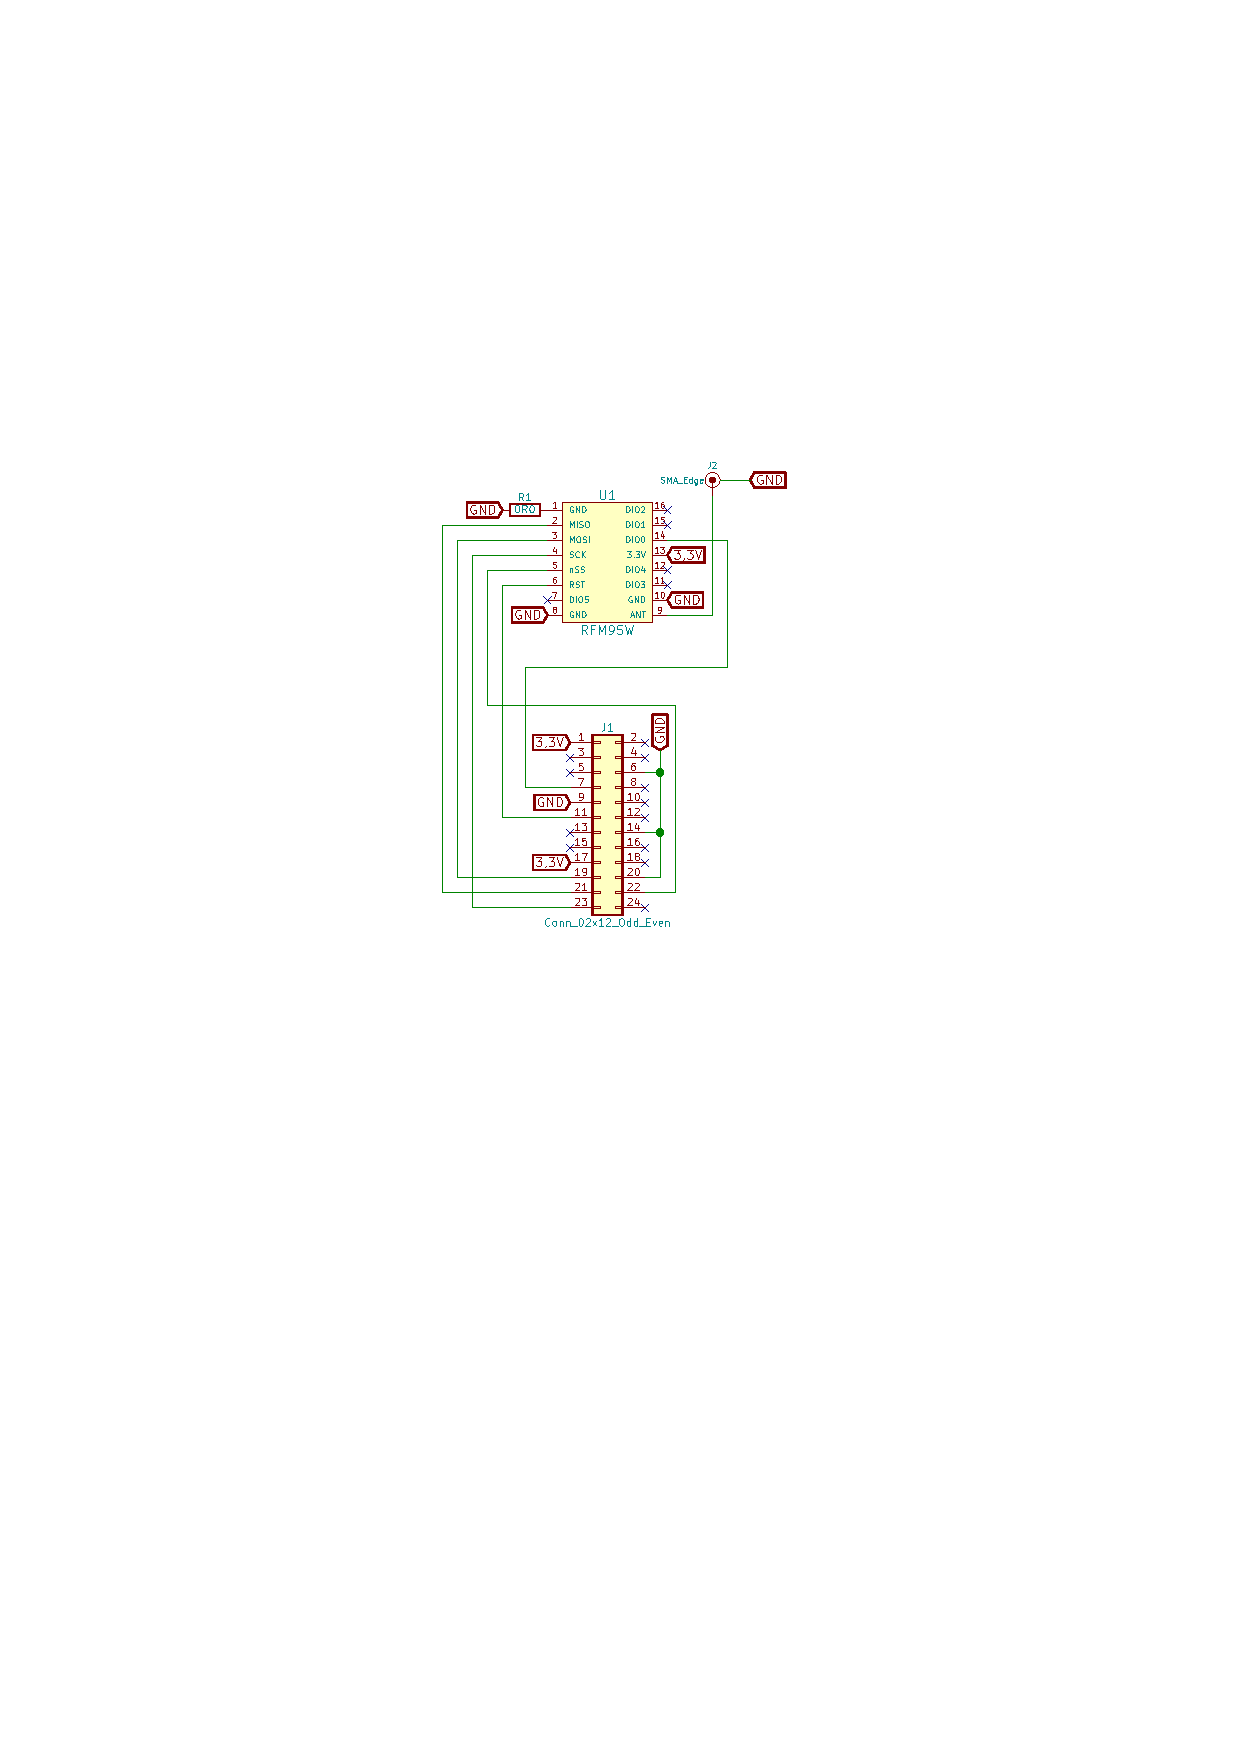
\includegraphics[ width = 0.6\textwidth]{HW_PART/Figs/KICKAD/gw.pdf}
            \caption {Schéma zapojení RFM95W do Raspberry Pi.}
            \label{figure:scheme_02}
    \end{figure} 
    
%CHECK ~
%CHECK red
%CHECK ...

